%--------------------------------------------------------------
% proposedModels.tex (use thesis.tex as main file)
%--------------------------------------------------------------
\chapter{Methodology}
\label{approaches}
%--------------------------------------------------------------

This chapter describes the GNN architectures for edge-level money laundering detection proposed in this dissertation.
We will propose a total of six different models; Graph Attention Networks (GAT, Section~\ref{sec:gat}) and Graph Isomorphism Networks (GIN, Section~\ref{sec:gin}) will be used as evaluation baselines;
Graph Transformers (GPSConv, Section~\ref{sec:gps}) will be then introduced to overcome the limitations (Section~\ref{sec:mp_limits}) of the two previous models;
Finally we will consider the architecture proposed in the paper Group-Aware Graph Neural Network ~\cite{mainpaper} (Section~\ref{sec:gagnn}) which, by aggregating nodes that are involved in suspicious transactions into gangs, and running a GNN on the obtained grouped graph, tries to detect money laundering organizations. 
we will consider three variants of the model one based on a GAT, one based on a GIN and one based on a Graph Transformer.

\section{Building the Financial Graph}
Before describing the models we define how the graph itself is built . Since the IBM AMLSim Dataset account (Node) features are very limited, we will leverage the transaction (Edge) features to derive the Node's ones.

Let \(\mathcal{N}(i)\) be the set of neighbors of account \(i\), \(e_{ij}\) the features vector of a transaction from account \(i\) to account \(j\), \(y_{ij}\) the label of that transaction. The feature vector \(x_i\) for the account \(i\) and his ground truth label \(\widehat{y_i}\) are defined as follows.
\begin{equation}
    x_i = \frac{1}{|\mathcal{N}(i)|} \sum_{j \in \mathcal{N}(i)} e_{ij}
\end{equation}
\begin{equation}
  \widehat{y_i} = \frac{1}{|\mathcal{N}(i)|} \sum_{j \in \mathcal{N}(i)} y_{ij}
\end{equation}
It's important to mention that in case of qualitative edge features or multiclass edge labels, the mean will be computed on the one-hot encoded vectors.

%--------------------------------------------------------------
\section{Graph Attention Networks}
\label{sec:gat}
%--------------------------------------------------------------

As mentioned in Section \ref{sec:GNNintro} different types of GNNs are defined by different AGGREGATE and UPDATE functions.

Graph Attention Networks introduce learned attention coefficients to improve the fixed weight aggregation of classical graph convolutions, allowing the model to understand which neigbours are more relevant torwards the classification task \cite{velickovic2018gat}.
The AGGREGATE function is defined as:
\begin{equation}
  m_i^{(k)} = \Vert_{t=1}^{H} \sum_{j \in \mathcal{N}(i)} \alpha_{ij}^{(k,t)} W^{(k,t)} h_j^{(k-1)}
\end{equation}
where \(H\) is the number of attention heads, \(\mathcal{N}(i)\) is the set of neighbors of node \(i\), \(W^{(k,t)}\) is the weight matrix for the attention head \(t\) at layer \(k\) and \(\alpha_{ij}^{(k,t)}\) is the attention coefficient between node \(i\) and its neighbor \(j\) at layer \(k\) and head \(t\) defined as
\begin{equation}
  \alpha_{ij}^{(k,t)} = \frac{\exp\left( e_{ij}^{(k,t)} \right)}{\sum_{l \in \mathcal{N}(i)} \exp\left( e_{il}^{(k,t)} \right)}
\end{equation}
where, in our case, the unnormalized attention scores \(e_{ij}^{(k,t)}\) also rely on the edge features \(\ell_{ij}\) of the edge \((i,j)\).
\begin{equation}
  e_{ij}^{(k,t)} = \operatorname{LeakyReLU}\left( \mathbf{a}^{(k,t)^\top} \left[ W^{(k,t)} h_i^{(k-1)} \;\; W^{(k,t)} h_j^{(k-1)} \;\; W_e^{(k,t)} \ell_{ij} \right] \right)
\end{equation}
where \(\mathbf{a}^{(k,t)}\), \(W^{(k,t)}\) and \(W_e^{(k,t)}\) are learnable parameters.

The UPDATE function is then defined as:
\begin{equation}
  h_i^{(k)} = \begin{cases}
    \operatorname{ReLu}\!\left( m_i^{(k)} \right)
      & k < L \\
    \operatorname{Id}\!\left(
      \dfrac{1}{H} \displaystyle\sum_{t=1}^{H}
      \sum_{j \in \mathcal{N}(i)} \alpha_{ij}^{(k,t)}\,
      \mathbf{W}^{(k,t)} h_j^{(k-1)}
    \right) & k = L
  \end{cases}
\end{equation}
Notice how the UPDATE function is different for the last layer. This is due to the fact that it averages the single heads outputs to produce an embedding of dimension $d_{\text{out}}$ instead of concatenating them; which is the case for intermediate layers.

The embeddings are then leveraged for edge classification. Let \((i,j)\) be an edge, his final representation will be the concatenation of the embedding of the source node \(h_i^{(L)}\), the embedding of the destination node \(h_j^{(L)}\) and the feature vector \(\ell_{ij}\). \([h_i^{(L)}, h_j^{(L)},\ell_{ij}]\) is then passed through a Multi-Layer Perceptron that computes the prediction.

%--------------------------------------------------------------
\section{Graph Isomorphism Networks}
\label{sec:gin}
%--------------------------------------------------------------
Graph Isomorphism Networks achive the theoretical upper bound of expressive power for message passing GNNs \cite{xu2019gin}. By using a MLP in the update function instead of a simple linear transformation, they are able to match the expressive power of the 1-Weisfeiler-Lehman test (Definition \ref{def:wl}).
The AGGREGATE function is simply defined as:
\begin{equation}
  m_i^{(k)} = \sum_{j \in \mathcal{N}(i)} h_j^{(k-1)}
\end{equation}

The UPDATE function, which is what actually differentiate GIN from other GNNs, is defined as:
\begin{equation}
  h_i^{(k)} = \operatorname{MLP}^{(k)}\!\left( \left(1 + \varepsilon^{(k)}\right) h_i^{(k-1)} + m_i^{(k)} \right)
\end{equation}
where \(\varepsilon^{(k)}\) is a learnable parameter. In our implementation, we used a two-layer MLP with a ReLU activation:
\begin{equation}
  \operatorname{MLP}(z) = W_2\,\operatorname{ReLU}\!\left(W_1 z + b_1\right) + b_2
\end{equation}
where \(W_1\), \(W_2\), \(b_1\) and \(b_2\) are learnable parameters.
The embeddings are then leveraged for edge classification in the same way as for GAT.

%--------------------------------------------------------------
\section{Limitations of Local Message Passing}
\label{sec:mp_limits}
%--------------------------------------------------------------
GATs and GINs, both belonging to the family of local message passing GNNs, share common limitations.
\subsection{Weisfeiler-Leman test upperbound}
Theoretically it has been proved that the expressive power of local message passing GNNs is upper bounded by the 1-Weisfeiler-Leman test ~\cite{xu2019gin};
\begin{definition}[Isomorphic Graphs]
  Two graphs \(G=(V,E)\) and \(G'=(V',E')\) are isomorphic if there exists a bijection \(f: V \to V'\) such that for all \(u,v \in V\), \((u,v) \in E \Longleftrightarrow (f(u),f(v)) \in E'\).
\end{definition}
\begin{definition}[1-Weisfeiler--Leman test]
\label{def:wl}
The 1-Weisfeiler-Leman (1-WL) test is an algorithm to determine whether two graphs \(G=(V,E)\) and \(G'=(V',E')\) are isomorphic or not. It works by iteratively assigning colours to nodes according to the local structure of the graph. The process is defined as follows:
\begin{enumerate}
    \item \textbf{Initialization}: Every node it's initialised with the same color \(c_i^{(0)}=c^{(0)} \; \forall i\in V,V'\);
    \item \textbf{Iteration}: At each step \(k\), each node updates its colour by collecting the colours of all its immediate neighbours and combining them with its current colour to create a new one:
    \begin{equation}
      c_i^{(k)} = \operatorname{HASH}\!\left(c_i^{(k-1)},\, \left\{\!\left\{ c_j^{(k-1)} : j \in \mathcal{N}(i) \right\}\!\right\}\right)
    \end{equation}
    the \(\operatorname{HASH}\) function guarantees that different combinations of colours will always produce a new distinct colour.
    \item \textbf{Comparison}: After each step, the algorithm compares the number of nodes for each colour in both graphs. If they are different, we are certain that the graphs are not isomorphic. Unfortunately, if the colours stop updating and the sets are still identical, the test is inconclusive; there is no guarantee that the two graphs are actually isomorphic.
    In Figure \ref{fig:wl} we can see an example of non-isomorphic graphs that are not discriminated by the 1-WL test.
\end{enumerate}
\begin{figure}
  \centering
  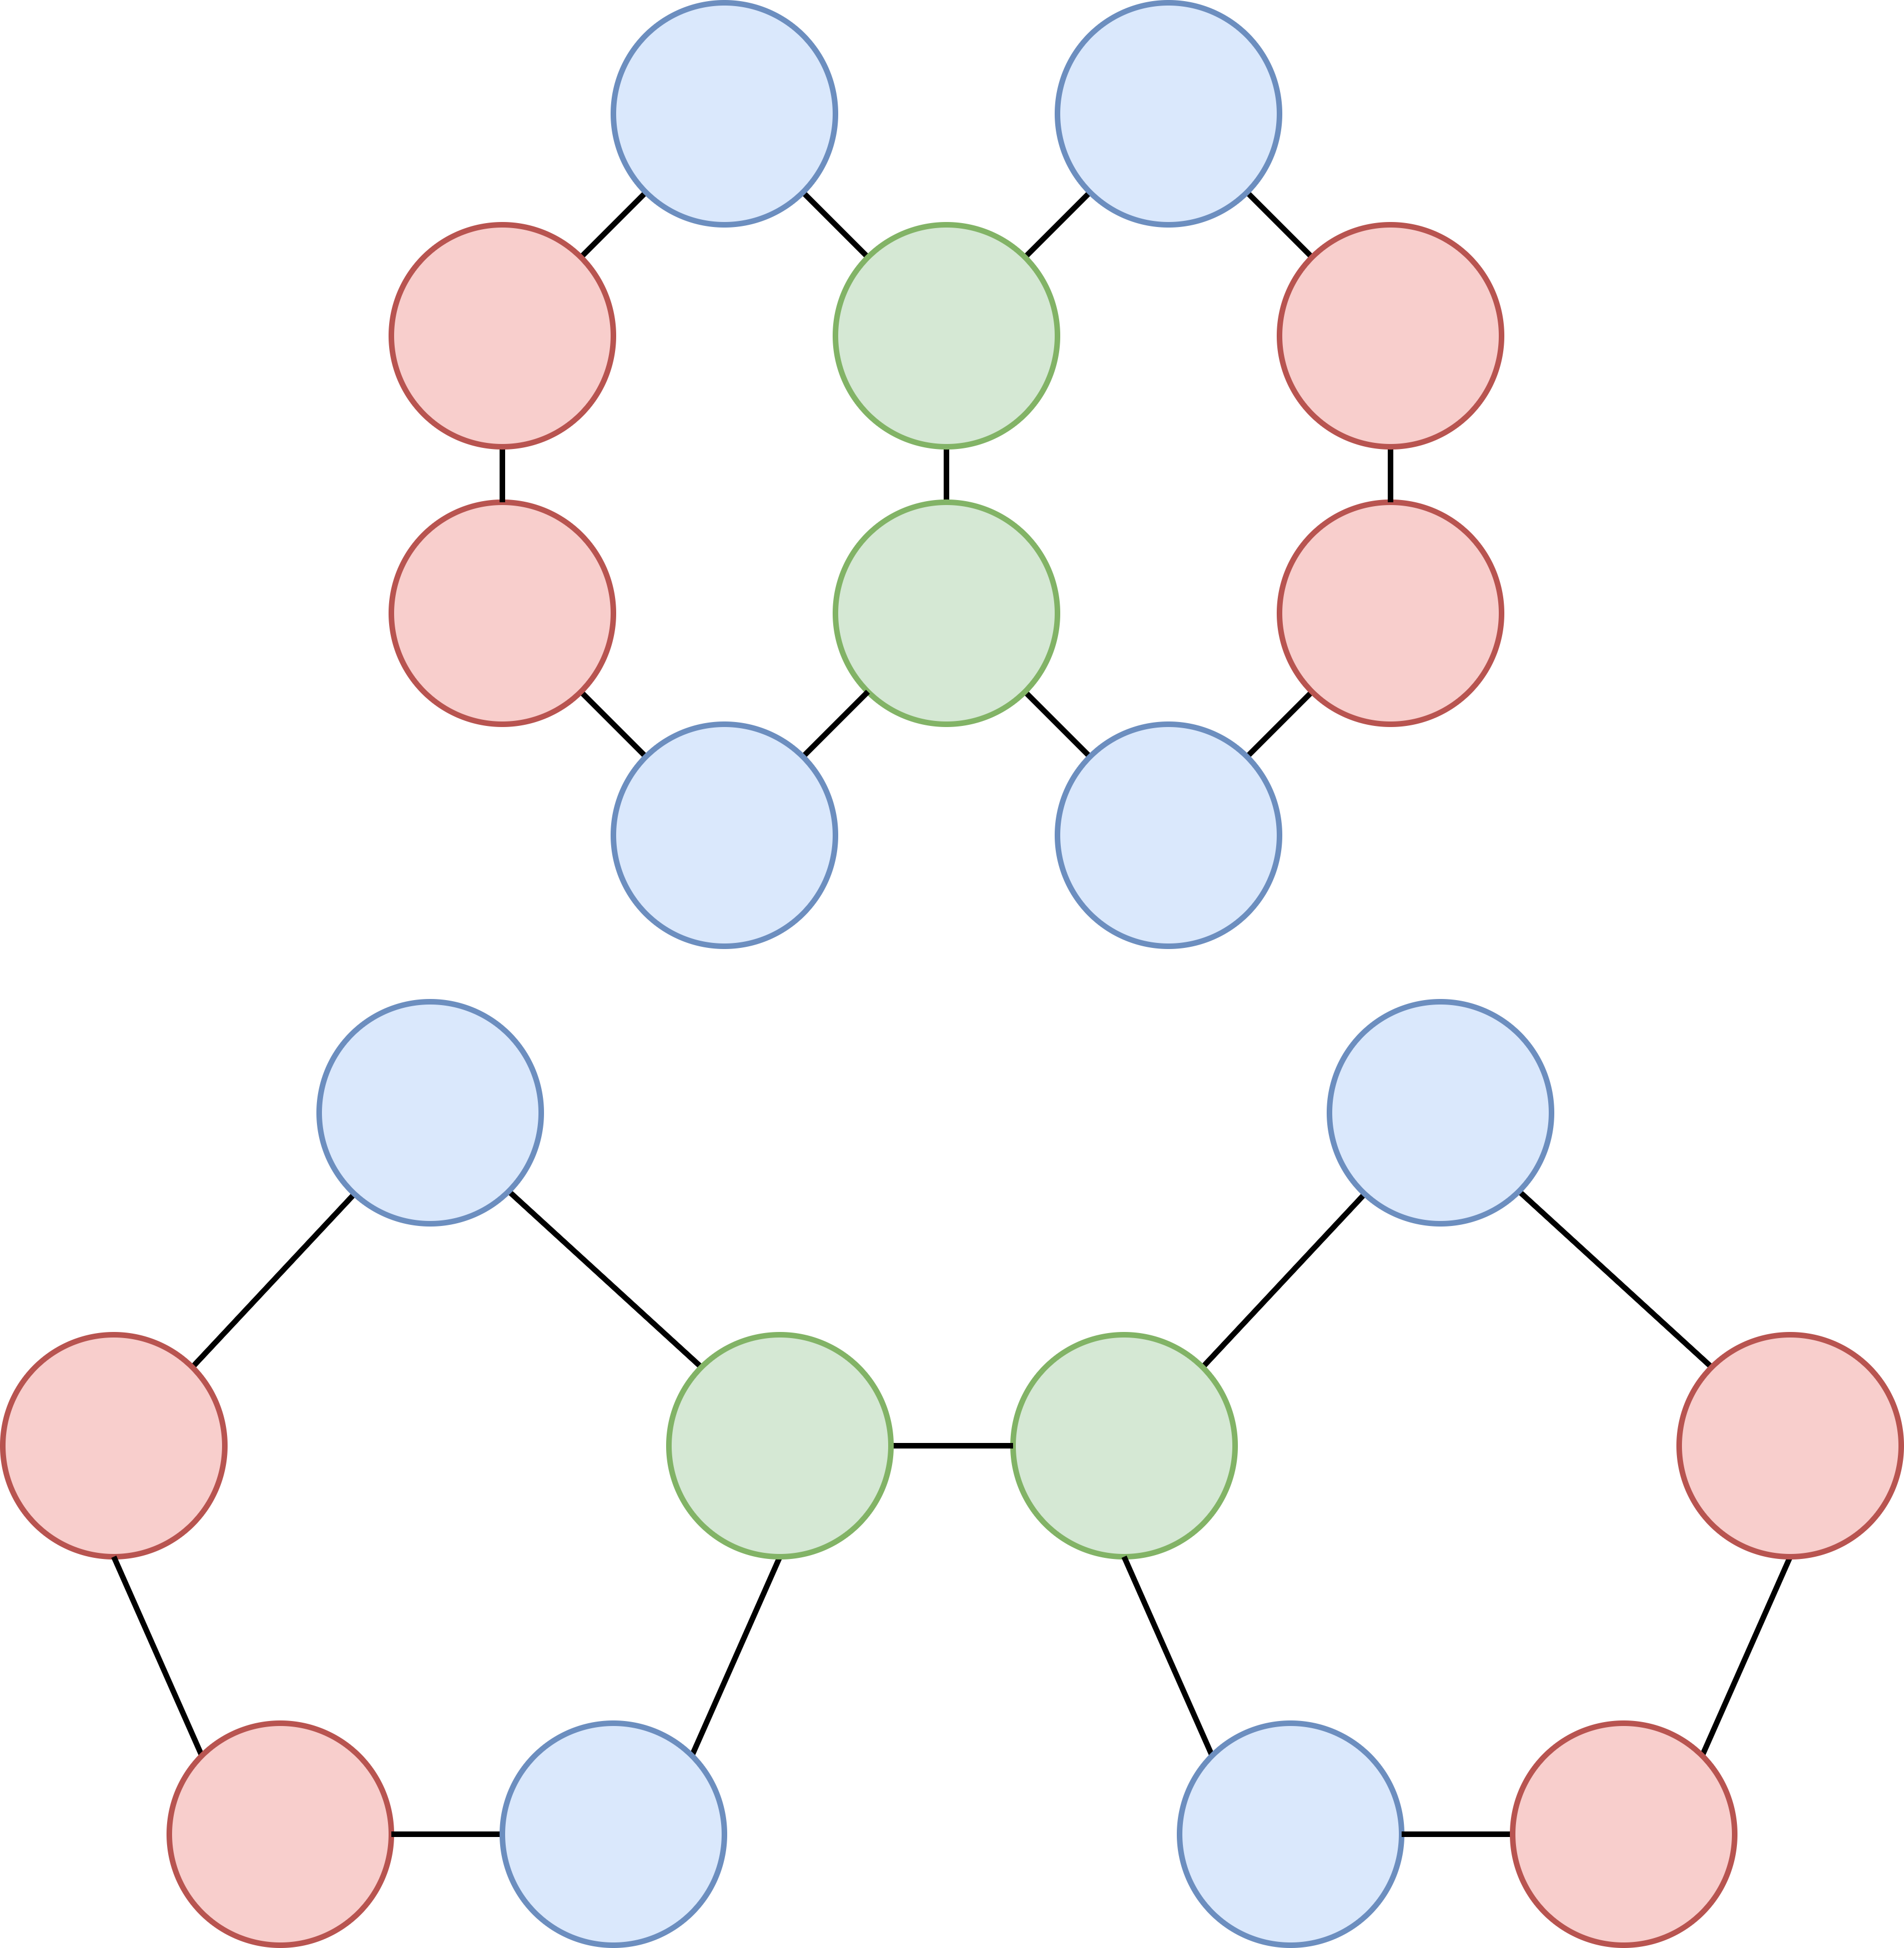
\includegraphics[width=0.8\textwidth]{IMG/wllimits.png}
  \caption{Non-isomorphic graphs that are not discriminated by the 1-WL test}
  \label{fig:wl}
\end{figure}
\end{definition}
This means that message passing GNNs are unable to discriminate certain non-isomorphic graph structures, limiting their ability to detect global topological patterns.

\subsection{Oversmoothing}
Growing the number of layers \(L\) in a GNN generally allows to capture higher order and more complex dependencies. However, as \(L\) grows, node embeddings tend to converge to a stationary point that is virtually identical for all nodes~\cite{Cheng_2025}.
When this happens, the node embeddings lose their ability to represent different nodes and the model loses its discriminative power.

\subsection{Oversquashing}
To capture interactions between nodes separated by a distance $r$, GNNs require at least $r$ layers of message passing. 

While the receptive field $\vert{}\mathcal{N}_r(v)\vert{}$ grows exponentially with $r$, the representation $h_v \in \mathbb{R}^d$ maintains its fixed capacity $d$. Consequently, propagating signals across multiple hops forces an exponentially increasing volume of neighborhood information into a fixed-size vector, creating an informational bottleneck.

This gets worse across graph bottlenecks, where signals from distant nodes $u$ are heavily diluted and fail to influence the final embedding of $v$.
~\cite{Cheng_2025}.
\bigskip

To overcome those limits we propose two possible solutions. Graph Transformers (Section~\ref{sec:gps}), adding global attention to the message passing mechanism, and Group-Aware GNNs (GAGNNs) \cite{mainpaper} (Section~\ref{sec:gagnn}), introducing a clustering mechanism to merge nodes that are suspected to be doing ML toghether and predicting their labels as a groups.

%--------------------------------------------------------------
\section{Graph Transformers}
\label{sec:gps}
%--------------------------------------------------------------

Graph Transformers leverage the transformers self-attention mechanism to enrich the local message passing mechanism with global context awareness. 
In this work we adopt the \emph{General, Powerful, Scalable} (GPS) architecture ~\cite{rampasek2022gps}, implemented in PyTorch Geometric as \texttt{GPSConv}.
The main idea is to combine, within each layer, local message-passing toghether with global self-attention, allowing the model to capture both local structural information and long-range dependencies.

\subsection{GPSConv Layer}
In each GPSConv layer the node embeddings are updated by two parallel procedures, local message passing and global attention; the two outputs are then combined to produce the final output. 

\paragraph{Local Message Passing}
The local message passing is performed by a Graph Isomorphic Network (GIN), as the one presented in Section~\ref{sec:gin}.
\begin{equation}
  h_i^{\text{local},(k)} = \operatorname{MLP}_{\text{local}}^{(k)}\!\left(
    \left(1 + \varepsilon^{(k)}\right) h_i^{(k-1)}
    + \sum_{j \in \mathcal{N}(i)} h_j^{(k-1)}
  \right)
\end{equation}

\paragraph{Global Attention}
A standard multi-head self-attention module is applied over all nodes, capturing long-range interactions without the locality constraint of message passing:
\begin{equation}
  h_i^{\text{global},(k)} = \operatorname{MHA}^{(k)}\!\left(
    h_i^{(k-1)},\;\left\{h_j^{(k-1)}\right\}_{j \in V}
  \right)
\end{equation}
with $H$ parallel attention heads.
\bigskip

The outputs of both branches are then summed toghether to obtain the final node representation:
\begin{equation}
  h_i^{(k)} = h_i^{\text{local},(k)} + h_i^{\text{global},(k)}
\end{equation}

\subsection{Input/Output Projections}

GPSConv operates with a fixed channel dimension $d_h$ across all layers.
Since the original node features $x_i \in \mathbb{R}^{d_{\text{feat}}}$ and
the desired output dimension $d_{\text{out}}$ generally differ from $d_h$,
two linear projections are added:
\begin{align}
  \tilde{x}_i &= W_{\text{in}}\, x_i, \quad W_{\text{in}} \in \mathbb{R}^{d_h \times d_{\text{feat}}} \\
  X^{(L)} &= W_{\text{out}}\, H^{(L)}, \quad W_{\text{out}} \in \mathbb{R}^{d_{\text{out}} \times d_h}
\end{align}
where $H^{(L)} \in \mathbb{R}^{N \times d_h}$ is the matrix containing the final node embeddings $h_i^{(L)}$ for nodes after the $L$-th layer.
Notice that the constraint $d_h \bmod H = 0$ must be satisfied to allow MHA to split the embedding evenly across attention heads.

The intermediate representations produced by each head are then concatenated along the feature dimension and linearly projected to form the final multi-head attention output.

By combining local GIN message passing with global multi-head self-attention, GPSConv overcomes the WL ceiling and oversquashing.

%--------------------------------------------------------------
\section{Group-Aware Graph Neural Networks}
\label{sec:gagnn}
%--------------------------------------------------------------

As introduced in Section~\ref{moneyLaundering}, money laundering is inherently an organized crime. Illicit transactions are not isolated events scattered randomly across the graph, but are rather concentrated among clusters of colluding accounts acting as gangs \cite{mainpaper}. Detecting fraud solely at the node or edge level tends to ignore this crucial group structure. 

To overcome these limitations, we adopt the \emph{Group-Aware Graph Neural Network} (GAGNN) architecture proposed by Cheng et al. \cite{mainpaper}. GAGNN is a multi-component pipeline that can embed any of the previously described GNNs (GAT, GIN, or GPSConv) as backbone and enriches them with two key mechanisms:
\begin{enumerate}
  \item An \emph{eMRF layer} (Edge Markov Random Field) that encourages nodes involved in the same fraud ring to receive similar embeddings.
  \item A \emph{Group Representation Layer} that explicitly detects and groups suspicious accounts into super-nodes, adding a community-level classification.
\end{enumerate}

The overall GAGNN pipeline proceeds in five steps.

\subsection{Community-Centric Encoder}
\label{sec:encoder}
The first step employs a standard GNN backbone (GAT, GIN, or GPSConv) to transform the raw node feature matrix $X^{(1)} \in \mathbb{R}^{N \times d_{\text{feat}}}$ into enriched embeddings $X^{(2)} \in \mathbb{R}^{N \times d_{\text{out}}}$ by stacking $L$ message passing layers;
\begin{equation}
  X^{(2)} = f_{\text{GNN}}^{(L)}\!\left(\cdots f_{\text{GNN}}^{(1)}\!\left(X^{(1)}, E\right)\cdots\right)
\end{equation}
where $E$ denotes the set of edges. A classifier then uses these embeddings to produce a preliminary node-level prediction $p_{\text{fraud}}$, which will be utilized by the subsequent eMRF layer;
\begin{equation}
  p_{\text{fraud}} = \sigma\!\left(W_c\, X^{(2)}\right) \in [0,1]^{N}
\end{equation}
where $\sigma$ is the sigmoid activation function. Notice that $p_{\text{fraud}}$ represents the probability of a node being illicit. Because the node classification step focuses strictly on detecting the presence of laundering, this prediction remains binary even in multiclass scenarios. The differentiation of specific laundering patterns is handled exclusively at the transaction level later in the pipeline.

\subsection{Edge Markov Random Field Layer}
\label{sec:emrf}
The eMRF layer refines the embeddings $X^{(2)}$ by pulling together nodes that belong to the same community and repelling those that do not. This community similarity is derived from both the graph topology and the node attributes.

First, the topological similarity $\varepsilon(v_i, v_j)$ measures how much more connected nodes $v_i$ and $v_j$ are compared to the average connection density of a random graph:
\begin{equation}
  \varepsilon(v_i, v_j) = \frac{d_i\, d_j}{2|E|} - a_{ij}
\end{equation}
where $d_i$ is the degree of node $v_i$, $|E|$ is the total number of edges, and $a_{ij}$ is the adjacency indicator; $a_{ij} = 1$ if an edge exists between $v_i$ and $v_j$ and $0$ otherwise. Next, the attribute similarity is computed as the normalized cosine similarity between the intermediate embeddings:
\begin{equation}
  R_\zeta(v_i, v_j) = \operatorname{Normalize}\left( \frac{h_i^{(2)^\top}\, h_j^{(2)}}{\|h_i^{(2)}\|\;\|h_j^{(2)}\|} \right)
\end{equation}
These two measures are linearly combined via a trade-off parameter $\beta$:
\begin{equation}
  \gamma(v_i, v_j) = \beta\,\varepsilon(v_i, v_j) + (1 - \beta)\,R_\zeta(v_i, v_j)
\end{equation}

Nodes predicted to belong to the same class by the coarse classifier are attracted, while nodes of different classes are repelled. The pairwise potential $\Psi(v_i, v_j)$ is defined as:
\begin{equation}
  \Psi(v_i, v_j) = (1 - 2\sigma(v_i, v_j)) \cdot \gamma(v_i, v_j)
\end{equation}
where $\sigma(v_i, v_j) = \mathbf{1}\!\left[ \lfloor p_{\text{fraud},i} + 0.5 \rfloor = \lfloor p_{\text{fraud},j} + 0.5 \rfloor \right]$ is a binary indicator of the same predicted class. Because the coarse node classifier is strictly binary, this indicator remains mathematically identical whether the overarching task is binary or multiclass.

Notice that our implementation differs mathematically from the original paper formulation, which used an exponential sign term $(-1)^{\sigma(v_i, v_j)}$. Since the derivative of $a^x$ relies on $\ln(a)$, computing $\ln(-1)$ is mathematically undefined and causes PyTorch to output NaN gradients during the backward pass. We solved this by using the equivalent linear mapping $(1 - 2\sigma)$. Furthermore, since the hard threshold $\lfloor \cdot + 0.5 \rfloor$ is not differentiable, we utilize a Straight-Through Estimator (STE). During the forward pass, the model uses the hard indicator, while during the backward pass, gradients are propagated through a soft continuous approximation.

Finally, the refined embeddings $X^{(3)}$ are computed using a mean-field update:
\begin{equation}
  X^{(3)} = X^{(2)} - \Psi\, X^{(2)}\, H^{(2)}
\end{equation}
where $H^{(2)}$ is a learnable weight matrix.

\subsection{Node-Level Classification}
\label{sec:node_clf}
The refined embeddings $X^{(3)}$ are mapped to node-level classification logits by a two-layer Multi-Layer Perceptron (MLP):
\begin{equation}
  p_{\text{node}} = \operatorname{MLP}_{\text{node}}\!\left(X^{(3)}\right)
\end{equation}
These logits provide the first of three supervision signals used to train the network.

\subsection{Group Representation Layer}
\label{sec:group_layer}
This layer classifies individual edges and discovers the latent groups of colluding accounts.
First, for each directed edge $(i,j)$, the layer concatenates the source and destination embeddings with the raw edge features to compute the transaction probability:
\begin{equation}
  p_{\text{trans}}(e_{ij}) = \operatorname{MLP}_{\text{edge}}\!\left([X^{(3)}_i \;\|\; X^{(3)}_j \;\|\; \ell_{ij}]\right)
\end{equation}
Then we used this distribution to construct the communities graph.
Considering an edge \(e_{ij}\), the two accounts \(i\) and \(j\) will be grouped together with a probability equal to their predicted illicit probability $p_{\text{trans}}(e_{ij})$ or, if the edge is in the training set, we will simply use its label to decide whether to group together the two nodes or not. In the case of a multi-class classification task, this Bernoulli probability is computed as $1 - p_{\text{licit}}(e_{ij})$, effectively considering all illicit classes together. The resulting groups are then collapsed into single super-nodes whose feature vector is the mean of its members' original features. Two communities will be connected by an edge if at least one node from one community have an edge with a node in the other community; the edge features will be dropped mantaing only the information about the connectivity.

\begin{equation}
  \hat{x}_g = \frac{1}{|\mathcal{G}_i|} \sum_{v \in \mathcal{G}_i} x_v
\end{equation}
Each group \(\mathcal{G}\) is considered illicit if it contains more than one account, licit otherwise. Formally we define the group label as:
\begin{equation}
  \hat{y}_g = \begin{cases}
    1 & \text{if } |\mathcal{G}_i| > 1 \\
    0 & \text{if } |\mathcal{G}_i| = 1
  \end{cases}
\end{equation}

\subsection{Group-Level Encoding and Prediction}
The same Community-Centric Encoder from Step 1 is reused on this new group graph $\hat{G}$ with shared weights:
\begin{equation}
  \hat{X}^{(3)} = \operatorname{CommunityCentricEncoder}\!\left(\hat{X},\, \hat{E}\right)
\end{equation}
\begin{equation}
  p_{\text{group}} = \sigma\!\left(W_c\, \hat{X}^{(3)}\right)
\end{equation}
where $\hat{X}^{(3)}$ is the resulting group-level embedding, and $p_{\text{group}}$ is the final illicit probability prediction obtained by performing a classification step on these embeddings. Sharing weights enforces consistency between the node and group levels while keeping the parameter count low.

\subsection{Multi-Task Loss}
\label{sec:loss}
Unlike standard GNNs that optimize a single objective, GAGNN is trained jointly on three supervised signals. The total loss $\mathcal{L}$ is a weighted sum of the node-level, transaction-level, and group-level losses:
\begin{equation}
  \mathcal{L} = c_1\,\mathcal{L}_{\text{group}} + c_2\,\mathcal{L}_{\text{node}} + c_3\,\mathcal{L}_{\text{trans}}
\end{equation}
where \(c_1,c_2,c_3 \in \mathbb{R}^+\) are hyperparameters and \(\mathcal{L}_{\text{group}}\), \(\mathcal{L}_{\text{node}}\) and \(\mathcal{L}_{\text{trans}}\) are the group-level, node-level, and transaction-level losses, respectively. Since nodes and groups are strictly classified as illicit or legitimate, their losses are always weighted Binary Cross-Entropy (BCE) functions:
\begin{align}
  \mathcal{L}_{\text{node}} &= \operatorname{BCE}_w\!\left(p_{\text{node}},\; y_{\text{node}}\right) \\
  \mathcal{L}_{\text{group}} &= \operatorname{BCE}_w\!\left(p_{\text{group}},\; y_{\text{group}}\right)
\end{align}
For the transaction classification, $\mathcal{L}_{\text{trans}}$ is a BCE loss for binary tasks, and a Cross-Entropy (CE) loss for multiclass classification.
\begin{equation}
  \mathcal{L}_{\text{trans}} = \begin{cases}
    \operatorname{BCE}_w\!\left(p_{\text{trans}},\; y_{\text{trans}}\right) & \text{if binary task} \\
    \operatorname{CE}_w\!\left(p_{\text{trans}},\; y_{\text{trans}}\right) & \text{if multiclass task}
  \end{cases}
\end{equation}
The positive-class weight $w$ is tuned to penalize false negatives, in the finance sector detecting most of the frauds is more important than maximizing the accuracy. By optimizing this joint loss, the model learns to identify money laundering at the individual, transaction, and community levels simultaneously.

%--------------------------------------------------------------
% experiments.tex (use thesis.tex as main file)
%--------------------------------------------------------------
\section{Experimental Settings}

\subsection{Data Preparation}\label{dataprep}
Before feeding the data into our models, we performed a series of preprocessing steps to organize the original features and ensure numerical stability.

First, categorical attributes were transformed using One-Hot Encoding. This encoding strategy is particularly effective for our architecture because when features are averaged (to derive node features from edges, or to collapse communities into super-nodes) the one-hot vectors naturally translate into proportions, preserving meaningful semantic information.

To capture the temporal dynamics of financial behavior, we engineered new features from the provided timestamps. In particular, we applied a cyclic encoding (using sine and cosine transformations) to the hour of the day. This cyclic representation is crucial for preserving the daily periodicity of transactions without introducing artificial discontinuities (e.g., the jump from 23:59 to 00:00).

For the multiclass classification task, we required specific labels for the different money laundering patterns. We mapped illicit transactions to their specific typology using the provided dataset metadata. Since not all illicit transactions were annotated with this information, transactions lacking a specific pattern label were dropped from the multiclass analysis.

Finally, we normalized the continuous financial amounts. Because money laundering datasets are typically heavily skewed by extreme outliers (e.g., massive illicit transfers), standard normalization techniques are often inadequate. Therefore, we employed a Robust Scaler, which normalizes features using the median and the interquartile range (IQR), according to the following formula:
\begin{equation}
    x_{\text{scaled}} = \frac{x - Q_2(x)}{Q_3(x) - Q_1(x)}
\end{equation}
where $Q_2(x)$ is the median, and $Q_1(x)$ and $Q_3(x)$ are the 25th and 75th percentiles of the feature values, respectively. This ensures that extreme values do not distort the feature space.

\subsubsection{Train, Validation and Test Split}
Financial transaction graphs are inherently dynamic and time-dependent. Consequently, a random split of the dataset would inevitably cause future information to leak into the past, compromising the model's evaluation. To prevent this, the data must be split chronologically. This chronological division closely mirrors real-world scenarios, where a model is trained on historical data to predict the legitimacy of new, incoming transactions.

While Cheng et al.~\cite{mainpaper} divided their dataset sequentially by weeks, our dataset spans a much shorter time frame of just a single week. To adapt to this constraint, we selected specific timestamp thresholds to partition the data: transactions occurring before September 7, 2022 at 14:55:00 were assigned to the training set ($\approx 70\%$); transactions between this time and September 8, 2022 at 16:12:00 constituted the validation set ($\approx 10\%$); and all subsequent transactions were allocated to the test set ($\approx 20\%$).

To address the severe class imbalance typical of AML datasets, we applied a downsampling strategy on the training set. The process involved identifying all fraudulent and legitimate accounts across the graph. We then randomly sampled the legitimate accounts to match the exact count of fraudulent accounts, achieving a balanced 1:1 ratio. After selecting these nodes, the graph was pruned by discarding any transaction where either the sender or the receiver was not among the sampled accounts. This ensures class balance at the node level while preserving the topological connections between the remaining actors.

Crucially, to strictly prevent any form of data leakage, the feature standardization process was isolated. The Robust Scaler was fitted exclusively on the transactions belonging to the training split, and the resulting parameters ($Q_1, Q_2, Q_3$) were then used to independently transform the validation and test sets.

\subsection{Hyperparameters Selection}

\subsection{Model Selection and Training settings}
%--------------------------------------------------------------
% spiego come ho allenato i modelli